\subsubsection{\acrshort{lstm} model}

This model is the same as the basic recurrent model but replacing the recurrent layer with an \acrshort{lstm} layer which is more complex and allows the network to learn to use more information from the past as explained in section \ref{lstm_theory}. This recurrent layer has $128$ units and graphically the model can be represented as follows:

\begin{figure}[H]
    \centering
    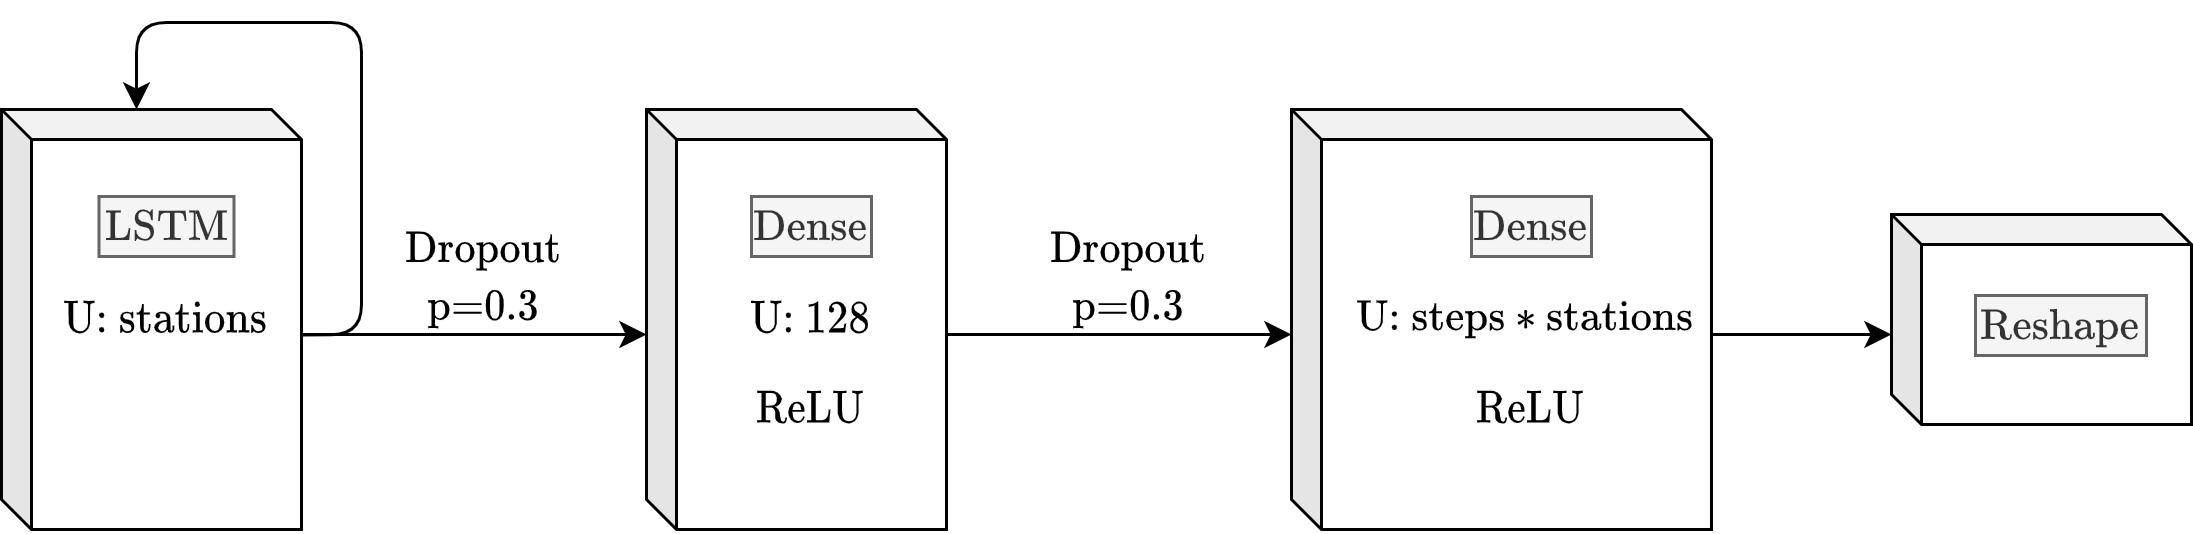
\includegraphics[width=12cm]{images/solution/models/LSTM.png}
    \caption{Recurring model \acrshort{lstm}}
    \label{fig:dense-model}
\end{figure}

As you can see it is the same model but replacing the \textit{SimpleRNN} layer by a \acrshort{lstm}. The code of this model has been defined as shown below:

\begin{minted}[fontsize=\scriptsize]{python}
from tensorflow.keras.models import Sequential
from tensorflow.keras.layers import Reshape, Dense, Dropout, Lambda, LSTM

# `steps` is a variable which has the number of intervals to be predict
steps = 0 

# `stations` is the number of stations in the bike network
stations = 0

lstm_model = Sequential([
    # LSTM layer
    LSTM(stations, return_sequences=False),
    
    Dropout(0.3),
    Dense(128, activation="relu"),
    
    # Output layer
    Dropout(0.3),
    Dense(steps * stations, activation="relu"),
    
    # Vector to matrix
    Reshape([steps, stations])
])
\end{minted}

The results of the model can be seen together with the other results in section \ref{results}.